\documentclass{article}
\usepackage[utf8]{inputenc}
\usepackage[spanish,es-tabla]{babel}
\usepackage[T1]{fontenc}
\usepackage{graphicx}
\usepackage{listings}

% Opciones

\title{Simanfor Basics}
\author{Moisés Martínez}

%%%%%%%%%%%%%%%%%%%%%%%%%%%%%%%%%%%%%%%%%%%%%%

\begin{document}
\maketitle

\section{Introducción}

Este documento describe el proceso de desarrollo de la nueva versión del simulador “Simanfor”. Esta nueva versión será desarrollada con el fin de desplegar el simulador en diferentes entornos de despliegue formados por nodos. Un nodo es un unidad básica de ejecución que estará formada por un procesador (n número de cores) y un conjunto de memria ram no distribuida. En base a esta definición se pueden definir tres posibles entornos:

\begin{itemize}
\item Entorno base: El simulador podrán desplegarse en un entorno local constituido por un único nodo. Este entorno permitirá la ejecución de las simulaciones consumiendo un mayor tiempo de ejecución. 
\item Entorno cloud: El simulador podrá desplegarse en diferentes nodos de manera que podrán acelerarse el tiempo de ejecución. Los diferentes nodos podrían tener diferentes características. 
\item Entorno Supercomputación: El simulador podrá desplegarse en entorno de supercomputación. Al igual que en el caso anterior, los diferentes nodos que forman el entorno podrán tener diferentes características, pero deberán compartir los diferentes sistemas de comunicación: (1) MPI; o (2) OpenMP. 
\end{itemize}

Además se utilizará una aplicación web que permitirá simplificar el proceso de interacción con el simulador. 

\section{Definición técnica}

En base a la información que hemos obtenido por parte de la Universidad de León, la estructura del nuevo simulador estaría formado por cuatro componentes que se pueden observar en la figura~\ref{fig:1}:

\begin{figure}[h]
\label{fig:1}
\caption{Arquitectura básica de funcionamiento del simulador}
\centering
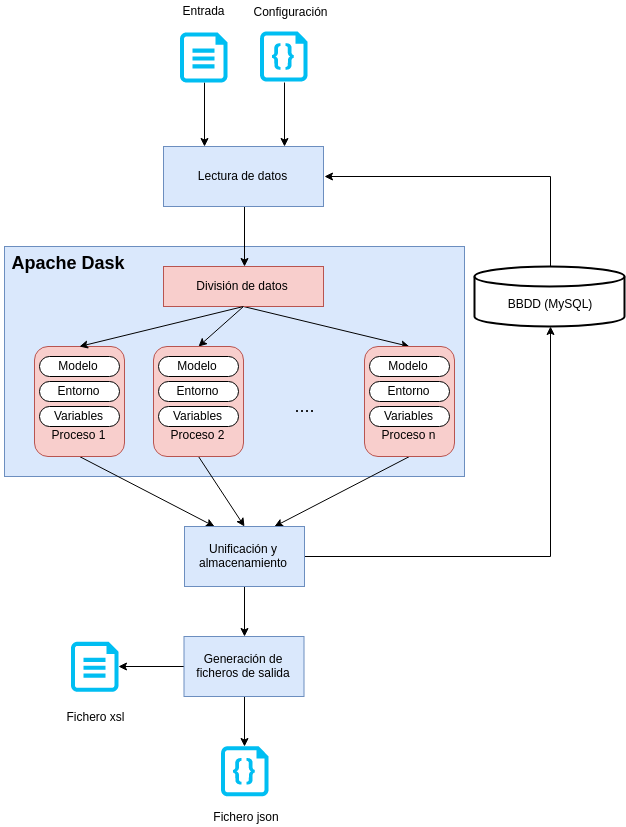
\includegraphics[scale=0.42]{./img/architecture.png}
\end{figure}

\begin{itemize}
\begin{item} Sistema de lectura de ficheros: Este sistema se ocupará de la configuración del entorno utilizando el fichero de configuración de entrada y el fichero de datos de entrada. 

\begin{itemize}

\item Fichero de entrada: Este fichero almacenará la información que utilizará el simulador para generar la salida. Su estructura se basa en la proporcionada por la universidad y se compone de un conjunto de filas y columnas (fichero xls) con información sobre las diferentes parcelas de terreno a simular. 

\item Fichero de configuración: Este fichero almacena la configuración del simulador. Esta información se divide en cuatro grupos: (1) información de conexión y almacenamiento para la definición de los conectores de bases de datos, fichero de logs y ficheros de resultado; (2) información referente al modelo a utilizar para generar la simulación; (3) información referente al entorno para la generación de la simulación (Esta información dependerá del modelo elegido); y (4) valores de las diferentes variables y constantes que utilizará el modelo. Parte de esta información puede estar almacenada en la base de datos relación.

\end{itemize}
\end{item}

\item Sistema de ejecución: El sistema de ejecución es el conjunto de procesos de ejecución que producirán la simulación que variará entre 1 y N. El número de proceso debe ser siempre inferior al número de nodos disponibles. Para la distribución de la información entre los nodos se utilizará Apache Dask, un sistema ligero de computación paralela para la manipulación de datos almacenados en tablas tabulares. Apache Dask ha sido seleccionado debido a su facilidad de uso y que la información utilizada en el proceso de simulación que puede modelarse como una tabla tabular. 

\item Sistema de unificación y almacenamiento: El sistema de unificación recogerá la información de cada uno de los nodos de ejecución y se almacenará en la base de datos. 

\begin{item} Sistema de generación de ficheros: El sistema de generación de ficheros almacenará la información en diferentes tipos de ficheros, que podrán ser almacenados en un repositorio con el fin de poder ser descargados a través de una aplicación web. El sistema generará dos tipos de ficheros de resultado:

\begin{itemize}
\item JSON: Un fichero de tipo JSON para la utilización de la información en otro tipo de aplicaciones de la nube. 
\item XSL: Un fichero de tipo XLS de formato muy similar al generado actualmente por el simulador. 

\end{itemize}
\end{item}

\end{itemize}

\end{document}